\chapter*{Problema B - Buscando un Hogar}

%\begin{center}
%  \begin{tabular}{ | l | l | l | }
%    \hline
%    Tiepo Límite: 2u & Memoria Límite: 512Mb & Código Fuente: \texttt{binarioseverywhere.\{java|cpp|c|py\}} \\
%    \hline
%  \end{tabular}
%\end{center}

Desde hace unos días, Moroni está buscando una nueva casa para su hámster, Schnitzel. Ha pasado gran parte de su tiempo intentando encontrar algo que le guste, pues Schnitzel es un ser realmente especial: únicamente acepta vivir en hogares que tengan la forma de un cuadrilátero convexo que además sea cíclico. Te voy a explicar por qué: A Schnitzel le gusta que rodeen su hogar con una pared circular, de manera que entre el cuadrilátero y el círculo se definan 4 áreas que sirvan como en patio de tu casa, como puedes ver en el siguiente dibujo.

\begin{center}
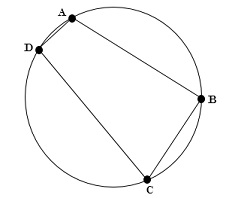
\includegraphics{CuadrilateroCiclico}
\end{center}

El problema es que Moroni ha encontrado innumerables casas con forma de
cuadrilátero, pero no sabe distinguir cuáles de ellas son como le gustan a 
Schnitzel. ¿Puedes ayudarlo?


\subsection*{Entrada}

La primera línea de entrada será un número entero $1 \leq T \leq 150$, que representará el número de casos de prueba. Cada caso estará separado por una línea en blanco y estará compuesto por cuatro líneas, para cada una de las cuales se ingresan dos números reales $x_i$, $y_i$ separados por un espacio, que representan las coordenadas de los vértices $A, B, C, D$ de la posible casa de Schnitzel, y cuyo orden corresponde a la dirección de las manecillas del reloj. 


\subsection*{Salida}

Para cada caso, imprime ``Schnitzel la acepta." si el cuadrilátero es de la forma que le gusta a la hámster; en otro caso imprime ``Sigue buscando, Moroni.".


\subsection*{Límites de los conjuntos de datos}

\begin{itemize}
\item Pequeño: $0 \leq |x_i|, |y_i| \leq 10^3$  $\quad \quad \quad$ 70 puntos.
\item Grande: $\,\;0 \leq |x_i|, |y_i| \leq 10^5$ $\quad \quad \quad$ 30 puntos.
\end{itemize}
\newpage

\begin{multicols}{2}

\subsection*{Entrada Ejemplo}
\begin{verbatim}
3
0 1
2 4
4 4
6 1

0 1
4 4
6 1
4.8 -1.239113

0 0
4 1
3 6
3 -2
\end{verbatim}
%41
\columnbreak

\subsection*{Salida Ejemplo}
\begin{verbatim}
Schnitzel la acepta.
Schnitzel la acepta.
Sigue buscando, Moroni.
\end{verbatim}
\end{multicols}

\subsection*{Notas:}
En caso de que quieras comparar dos números \texttt{a} y \texttt{b} de precisión flotante, en vez de hacer:

\texttt{if (a==b)} 

haz 

\texttt{if ( fabs(a-b)<=1e-4 )}

Esto debido a que los números flotantes no suelen tener una representación binaria exacta y se pierde precisión.

(\texttt{fabs} es la función que devuelve el valor absoluto de un valor flotante).